%\nonstopmode
\documentclass[a4paper, 12pt]{article}
\usepackage{verbatim,amsmath,graphicx,geometry,textcomp,url,caption,float,verbatim,parskip} %,parskip
\geometry{ a4paper, total={170mm,257mm}, left=20mm, top=20mm}
\usepackage[dvipsnames]{xcolor}
\definecolor{subr}{rgb}{0.8, 0.33, 0.0}

\begin{document}
\begin{center}
Demystifying neutron lethargy			\\
Ocean Wong								\\
2019-03-18
\end{center}

Consider the following question:

`` 
How can the average number of collisions necessary to thermalise a fission neutron (slow
it down from 2 MeV to 1 eV) in deuterium be calculated?
'' 

When deriving the number of collision required $N$ for a given $\alpha = (\frac{A-1}{A+1})^2$ (where $A$ is the atomic mass), several fellow students have stumbled across the following misconception:

\section{Incorrect method}\label{Incorrect}
An intutive method is to do the following:

\begin{align}
	\overline{E_f} &= \int P(E) E dE =  {E_i} \frac{(\alpha+1)}{2} \\
	\overline{\Delta u} &= ln \left( \frac{E_i}{\overline{E_f}} \right)	\\
	N &= \frac{ ln \left( \frac{2 MeV}{1eV} \right)} { \overline{\Delta u} }
\end{align}

Which corresponds to the procedure as follows:
\begin{enumerate}
	\item Find the average energy lost $\overline{E}$
	\item Calculate the lethargy change it represents
	\item Find the number of collisions (each with energy $\overline{E}$ lost) required to slow it down.
\end{enumerate}

In a single equation, this is represented as:
\begin{align}
	N&=\frac{u(2MeV) - 2(1eV)}{\Delta u \left(\int E P(E) dE \right) }\\
	N&=\frac{ln\left(2000000\right)}{ln\left(\frac{1+\alpha}{2} \right)}
\end{align}
Which gives the incorrect answer of 22.7 collisions for 2MeV neutrons moderated by Deuterium $A=2$

\section{Correct method} \label{Correct}
	However, the correct way to do so is 
\begin{align}
	\overline{\Delta u} &= \int (\Delta u) P\big(\Delta u \big) d(\Delta u)	\\
		&= \int\limits_{E_f=\alpha E_i}^{E_f=E_i} \Delta u (E_f) P\big(\Delta u (E_f) \big) \frac{d(\Delta u)}{dE_f} dE_f \label{scaleUprob}
\end{align}

where the conversion to $\Delta u$ is carried out as follows:
\begin{align}
	\Delta u (E_f) = ln\left(\frac{E_i}{E_f} \right)
\end{align}
and the probability distribution in $u$ space can be converted back into probability distribution in $E_f$ space in a straightforward manner:
\begin{align}
	P(E_f) dE_f &= P(\Delta u (E_f) ) {d(\Delta u)}	\\
	P(\Delta u (E_f) ) \frac{d(\Delta u)}{dE_f} &= P(E_f)
\end{align}
simplifying equation \ref{scaleUprob}
\begin{align}
	\overline{\Delta u} &=	\int\limits_{E_f=\alpha E_i}^{E_f=E_i} \big(\Delta u (E_f) \big) P\big(E_f \big) dE_f	\\
						&=	\int\limits_{E_f=\alpha E_i}^{E_f=E_i} ln \left( \frac{E_i}{E_f} \right) P\big(E_f \big) dE_f \\
\end{align}

Which will be evaluated to
\begin{align}
	\overline{\Delta u} &=	1+\frac{\alpha}{1+\alpha} ln(\alpha)	\\
	N &= \frac{ ln \left( \frac{2 MeV}{1eV} \right)} { \overline{\Delta u} }
\end{align}
Which gives 20.8 collisions for 2MeV neutrons moderated by Deuterium $A=2$

The numerical accuracy of this answer can be verified with the code
\begin{itemize}
	\item MonteCarlo.py
\end{itemize}

in the repository 
\begin{itemize}
	\item https://github.com/OceanNuclear/NeutronLethargy
\end{itemize}

\section{Explanation}
	The correct method does the following (Figure \ref{Fig1}):
	
	\begin{figure}[H]
	\centering
	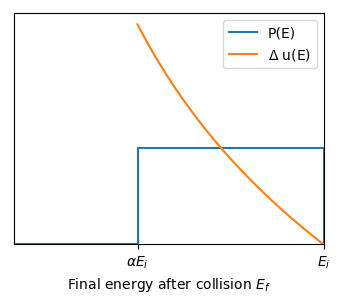
\includegraphics[height=5cm]{Fig1.png}
	\caption{Multiplying $P(E_f)$ by $\Delta u(E_f)$ gives a quantity with the dimension of `` Lethargy per unit energy'' .
	}\label{Fig1}
	\end{figure}
	
	Integrating $\Delta u(E_f) P(E_f)$ over $E_f$ gives the mean lethargy change $\overline{\Delta u}$.
	
	Alternatively, if one wishes to visualize it in terms of $\Delta u$,
	
	\begin{figure}[H]
	\centering
	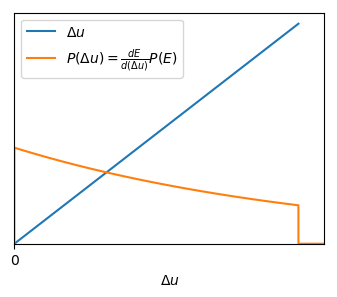
\includegraphics[height=5cm]{Fig2.png}
	\caption{Multiplying $P(\Delta u)$ by $\Delta u$ gives a dimensionless quantity. \\
	The probability density function as a function of $\Delta u$ is given by equation \ref{scaleUprob}.	}\label{Fig2}
	\end{figure}	

	Integrating $\Delta u P(\Delta u)$ over $\Delta u$ gives the mean lethargy change.


	Note that figure \ref{Fig1} is oriented in the opposite direction as figure \ref{Fig2}, neutrons starts with a high initial energy $E_i$ (RHS of figure \ref{Fig1})/ zero lethargy (RHS of figure \ref{Fig2}) $\Delta u=0$, and scatter down to lower energy/ greater lethargy, with the minimum energy achievable $= \alpha E_i$/ maximum lethargy gained $= ln(\alpha)$ in a single scatter.

	
	However, in section \ref{Incorrect}, the lethargy of the average average energy (green dotted line) is used instead.

	\begin{figure}[H]
	\centering
	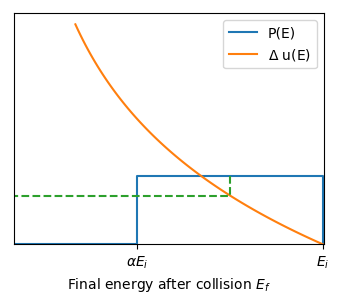
\includegraphics[height=5cm]{Fig3.png}
	\caption{The mid point of the rectangular probability density function is used, and the (wrong) mean lethargy change $\overline{\Delta u}$ is inferred from that.}\label{Fig3}
	\end{figure}		

	This will give an incorrect answer because the average $E_f$ as determined by the rectangular area is different from the average as determined by the area under the curve $ \Delta u P(\Delta u)$ (product of the two solid curves drawn).

	Due to the non-linearity of the $\Delta u(E)$ curve in figure \ref{Fig3} a small `excursion' to the left will contribute a much larger increment in lethargy gain than decrement in lethargy gain when there is a small `excursion' to the right.
	

	This means that a collision losing slightly more than $\overline{E}$ requires multiple collision losing slightly less energy than $\overline{E}$ to counter its effect.
	This problem is actually a confusion between arithematic mean (section \ref{Incorrect}) and geometric mean (section \ref{Correct}) in disguise. The former method falsely assumes that an arithmatic mean can be used, finding the arithmatic average of the energy lost $\Delta E = E_i-E_f$, instead of the geometric average of $\Delta E$ (which is identical to the arithmetic average of $\Delta u$).

	Note that if $\alpha$ is very close to 1, then this non-linearity can be ignored, i.e. at very large atomic masses, e.g. ${}^{238}$U, the above two methods should give very similar results.

\section{Physical intuition}
	Consider 4 hypothetical collisional events:

	\subsection{No variation in factor of energy loss}
	If all collisions scale down the energy by \emph{exactly} the same factor everytime, i.e. corresponding to the mid-point of the rectangular probability density distrbution (green line in figure \ref{Fig3}), then the lethargy lost calculated by both methods in section \ref{Incorrect} and \ref{Correct} will be the same.
	\begin{itemize}
		\item Factor of reduction in energy after each collisional event = \begin{verbatim}
			0.6, 0.6, 0.6, 0.6
		\end{verbatim}
		\item Total energy lost = $0.6^4 =  0.1296$
		\item Using section \ref{Incorrect} 's method : Energy lost = exp(4*ln(0.6)) = 0.1296
		\item Using section \ref{Correct} 's method: Energy lost = exp(ln(0.6)+ln(0.6)+ln(0.6)+ln(0.6)) = 0.1296
	\end{itemize}
	
	\subsection{Accounting for variation in factor of energy loss}
	However, using another set of hypothetical energy loss factors, with the same arithmatic average (0.6) as the set before, but with a non-zero standard deviation:
	\begin{itemize}
		\item Factor of reduction in energy after each collisional event = \begin{verbatim}
			0.5, 0.7, 0.5, 0.7
		\end{verbatim}
		\item Total energy lost = $0.6^4 =  0.1225$
		\item Using section \ref{Incorrect} 's method : Energy lost = exp(4*ln(0.6)) = 0.1296
		\item Using section \ref{Correct} 's method: Energy lost = exp(ln(0.5)+ln(0.7)+ln(0.5)+ln(0.7)) = 0.1225
	\end{itemize}
	This demonstrates how the numbers on the left hand side of the green line in figure \ref{Fig3} will skew the total energy lost towards a smaller value.
\section{Acknowledgement}
	Many thanks to Sam Dyson for his insight and discussion on this topic, as well as providing the inspiration for the last section.

\end{document}